\section{Interface avec le Reconnaisseur}

Cette partie du projet a pour objectif de lier la base d'apprentissage de notre logiciel avec le reconnaisseur choisi par l'utilisateur. Ainsi, cette partie étant très liée à l'utilisateur, il faut lui permettre de pouvoir facilement attacher le reconnaisseur de son choix au logiciel. C'est avec cette contrainte en tête que nous avons conçu l'architecture de cette partie.

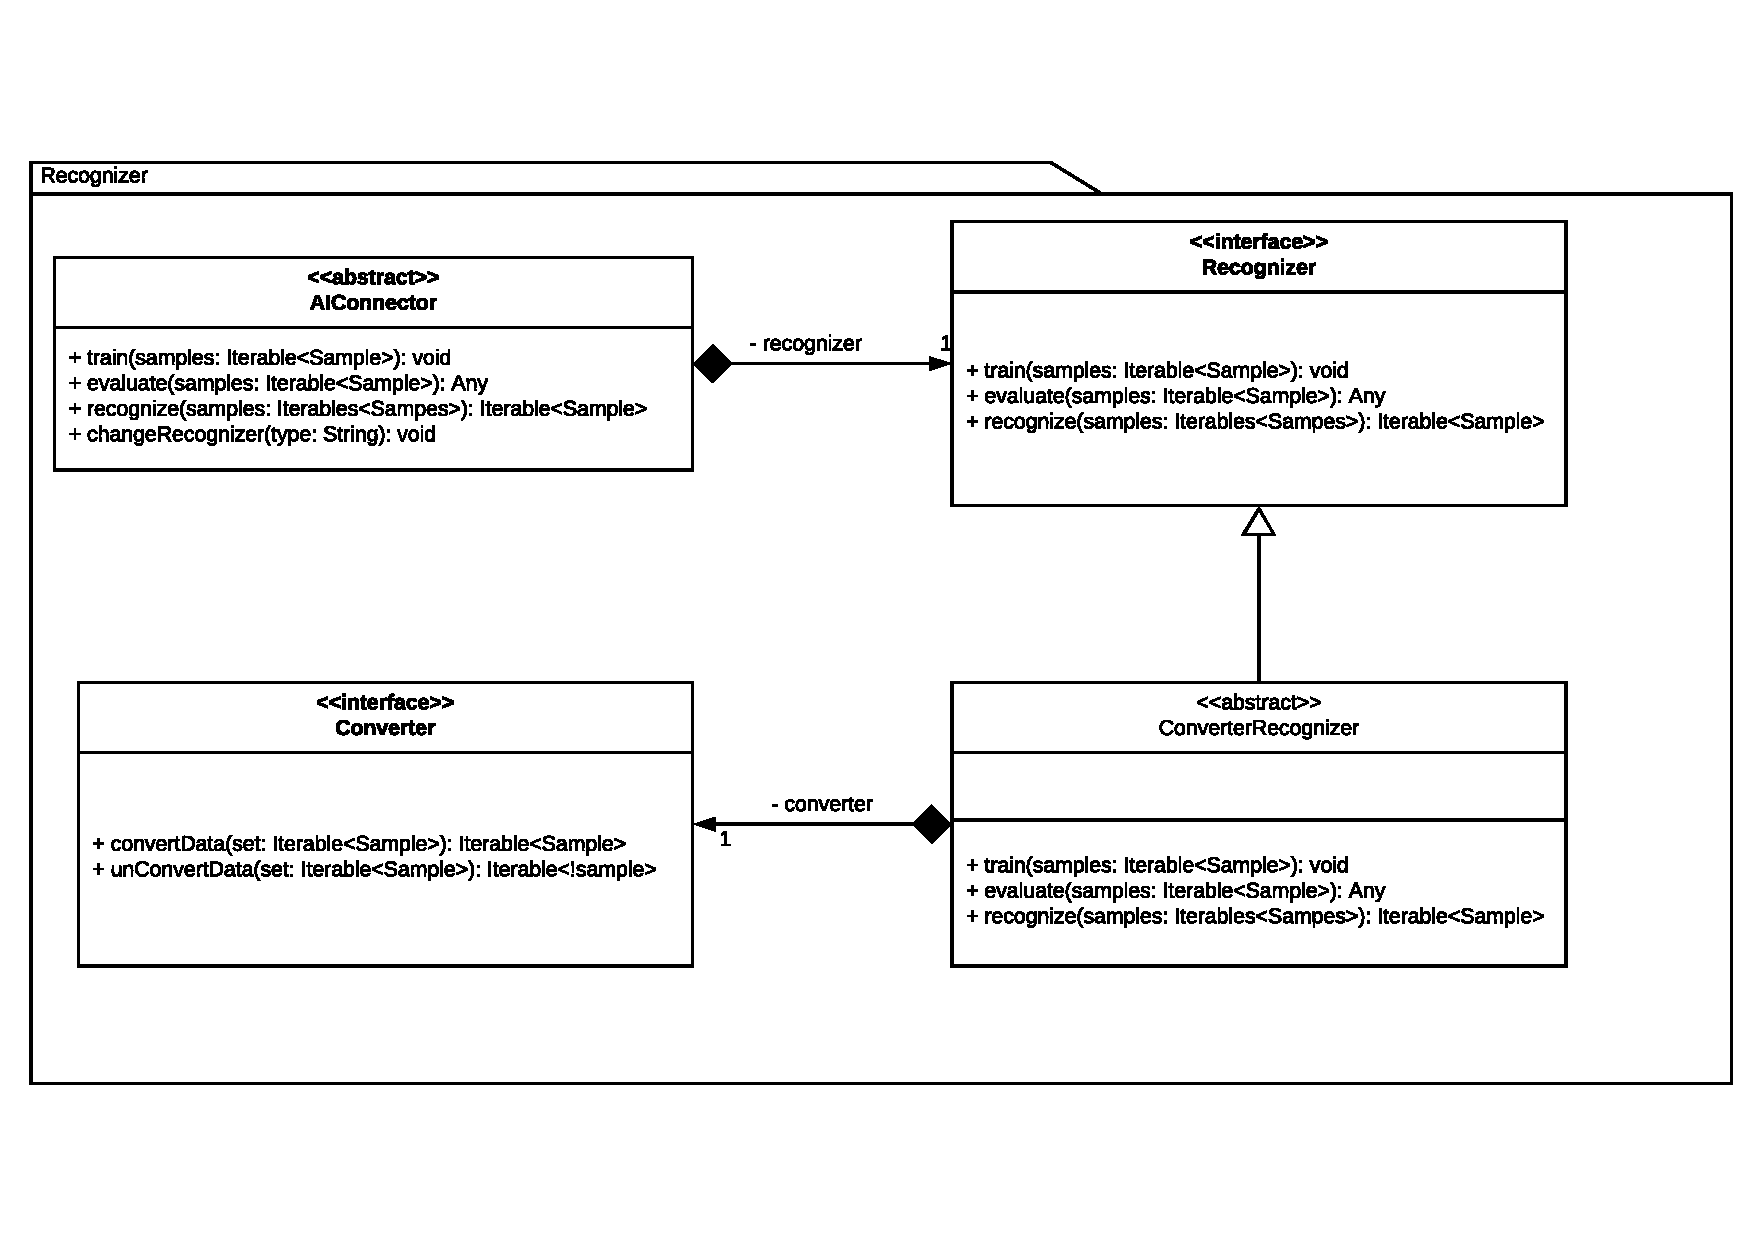
\includepdf[pages=-]{assets/UML_Recognizer}

\paragraph{Architecture}

